\documentclass[11pt]{article}
\usepackage[T1]{fontenc}
\usepackage{amsmath}   % Standard tools
\usepackage{amssymb}   % Math symbols
\usepackage{graphicx}  % Images
\usepackage{framed}    % "Framed" environment
\usepackage{tikz}
\usepackage{tikz-qtree}
\usetikzlibrary{calc}
\usepackage{cancel}
\usepackage{apacite}
\let\checkmark\origcheckmark
\usepackage{dingbat} % pointer arrow
\usepackage{utfsym}
\usepackage{fourier} % bomb

\title{\vspace{-3cm}Exploration of neural methods on English etymological classification}
\date{\today}
\author{Robin Huo \\ robin.huo@mail.utoronto.ca
\and Tim Logatsang \\ tim.logatsang@mail.utoronto.ca
\and Charles Wong \\ charleshm.wong@mail.utoronto.ca}

\graphicspath{{./IMAGES/}}

% ************ SECTION FORMAT ************ %

% ************ CUSTOM COMMANDS ********** %
%\newfontfamily\IPAfont[AutoFakeBold=1.5]{Times New Roman}
%\DeclareTextFontCommand{\ipa}{\IPAfont}
%
%\newfontfamily\unisymbols{DejaVu Sans}
%
%\newcommand{\cross}{\usym{2718}}
%\renewcommand{\checkmark}{\usym{2714}}

\begin{document}
	\maketitle
	
	\section{Introduction}
	
	Historical linguistics deals with different aspects of language change, one of which being etymology, the reconstruction and origin of words and other linguistic items. Traditional approaches to this field mostly involve looking at historical texts and tracing word formation and borrowings by linguists. The use of data-driven techniques is thus a lesser explored domain of research. The central observation motivating our approach is that patterns in morphology emerge as a result of borrowings from any specific language into another. As such, it may be possible to identify such classes of vocabulary within a language using statistical modelling, specifically using neural networks.
	
	In this paper, we assess the viability of using different neural network architectures in predicting the source language of borrowings into English. We compare CNN, RNN, and Encoder-only Transformer architectures. An important feature of our approach is that the inputs to all of these models are fixed-length character-level embeddings.
	
	Section \ref{sec:prob} of this paper further defines the problem space and some theoretical challenges. Section \ref{sec:summ} discusses prior work done in this area. Sections \ref{sec:meth} and \ref{sec:exp} describes our methodology, and presents our experiemental results. Section \ref{sec:conc} includes our conclusion and discussion of future work.
	
	\section{Problem definition} \label{sec:prob}        % define the problem (including brief motivation of solving this problem, and relevant dataset)
	Etymology is the study of the origin of words or other linguistic items.
	The term \textit{etymology} is also used to refer to a specific etymological origin.
	Generally speaking, words and linguistic structures are either borrowed or inherited.
	A linguistic item or construction is said to be borrowed if it is introduced into the language from an external language or variety, which provides the borrowed form.
	Borrowed words are also commonly called loanwords.
	For example, the English word \textit{pasta} is borrowed from the Italian word \textit{pasta}, which means pasta or noodles.
	Anything that is not borrowed is inherited.
	For example, the word \textit{word} has existed in English, in this or an earlier form, for as long as historical linguists can presently discern.
	
	Words of different origins may sometimes interact in different ways with the other systems of the language.
	For example, words of Latinate origin typically take the \textit{in-} prefix when deriving a negated form, e.g., \textit{in-validate}.
	On the other hand, native English words typically take the \textit{un-} prefix instead, e.g., \textit{un-lock}.
	Thus, knowing the etymology of the word can in some cases allow a speaker or system to more competently use language.
	
	It is common for words of different sources to display characteristic formal properties reflecting their origins.
	Thus, it is possible in some cases to predict the origin of a word given its form, to an extent.
	It is this problem that we wish to explore using neural techniques.
	Specifically, given an English word as input, we wish to predict the origin of the word given a set of predefined etymological classes.
	We will use the etymology-db \cite{etymologydb} dataset (more detail later) for etymological data.
	
	\section{Summary of prior work} \label{sec:summ}  % provide a brief summary of prior work
	
	While we are the first to apply such methods to etymological classification within the English language in particular, use of neural and deep learning methods to identify cases of lexical borrowing as well as the donor language has been explored in the past.
	
	\citeA{mi2016} uses recurrent neural networks (RNNs) to classify loanwords in Uyghur as originating from one of Chinese, Russian, and Arabic, achieving a macro-averaged F1 score of 0.7950. Later, \citeA{mi2018} uses convolutional neural networks (CNNs) with long short-term memory on the same problem to achieve an average F1 score of 0.8040.
	
	\citeA{miller2020} implements an RNN among other models in the task of predicting whether a word is borrowed or inherited across 41 different languages, with up to 2,000 words per language as training data, achieving an F1 score of 0.661. \citeA{miller2021} applies a simplified transformer model to the same task, achieving a lower F1 score of 0.559, but a shorter training time than the baseline based on RNNs.
	
	One of the authors previously submitted a project for CSC311, applying CNNs to achieve an F1 score of 0.83101 in classifying Korean nouns across nine different languages of origin.
	
	\section{Methodology} \label{sec:meth}
	
	We begin our investigation with the \textit{etymology-db} \cite{etymologydb} dataset, an open dataset compiled using Wiktionary's etymology data. It records up 31 different types of etymological relations, distinguishing between inheritance, borrowing, etc. For our purposes, we extracted the subset of relations with English, an approximate 36.6k entries. As one might expect, the distribution of related languages is extremely skewed. Of the 598 related languages recorded, the top 5 related languages (French, Latin, German, Italian, Spanish) account for 48.81\% of the dataset. This distribution is shown in Figure \ref{fig:zipf}, and it can be seen that it roughly follows Zipf's Law.
	\begin{figure}
		\centering
		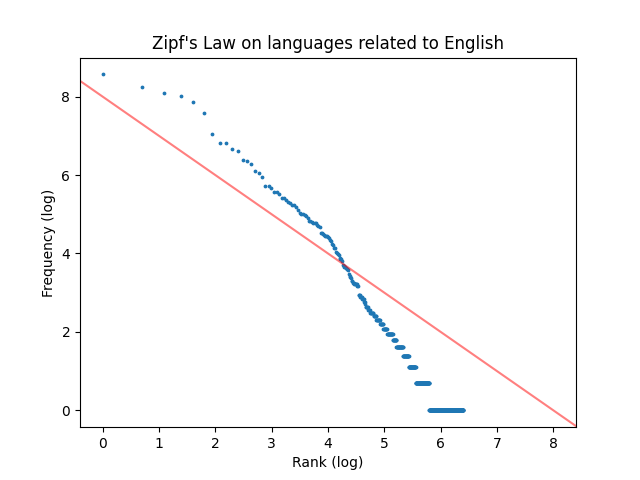
\includegraphics[scale=0.5]{zipf}
		\caption{Distribution of related languages in the \textit{etymology-db} dataset}
		\label{fig:zipf}
	\end{figure}
	In order for our models to be able to generalize well even to the lesser seen classes (i.e. related languages), we partitioned this data into training, validation, and test sets that were balanced with respect to class frequency.
	
	For each datapoint, we represent the input word using character-level embeddings. The embeddings for the 166 distinct characters used in the dataset were learned from scratch for each model separately. An alternate approach we considered was tokenizing words into morphemes instead. However, we opted for the character embeddings as we thought it allowed the potential for our models to learn more information about morpheme structure and specific phonotactic patterns. Tokenization also introduces complexity beyond just breaking up words into their orthographic character representations.
	
	\subsection{CNN}
	
	The main motivation for using a convolutional neural network was as a way to extract ``features" out of the character embedding representations such that they might resemble morphemes, or some higher level linguistic structure. Consider a hypothetical convolutional filter that is able to extract prefixes from the individual characters at the beginning of a word. Then should the input characters be the \textit{in-} prefix, the model might be able to confidently predict the related language to be Latin. In short, the convolutional filters are a way to condense the information encoded within a sequence of letters into larger and more meaningful units.
	
	\subsection{RNN}
	
	Fundamentally, the task at hand is to analyze a sequence and come up with a classification. As such, using a recurrent neural network, which is able to learn the relationships between a linear sequence of inputs, was an obvious choice. 
	
	\subsection{Transformer}
	
	Given our results using the recurrent neural network, it seemed a logical step to investigate using attention to tackle our problem. We take inspiration from the Transformers architecture first proposed by \citeA{attention} to build an Encoder-only classification model. The input word, transformed into its character embedding representation, is fed through a series of multi-headed self-attention layers, so that long distance relationships between characters can be learned. We learn positional encodings from scratch, and average pooling to generate a single output logit from the matrix of final attended representations of the individual characters.
	
	\section{Experiments and Results} \label{sec:exp}
	
	\section{Conclusion} \label{sec:conc}
	
	\bibliographystyle{apacite}
	\bibliography{citations}
\end{document}